% Options for packages loaded elsewhere
\PassOptionsToPackage{unicode}{hyperref}
\PassOptionsToPackage{hyphens}{url}
\PassOptionsToPackage{dvipsnames,svgnames,x11names}{xcolor}
%
\documentclass[
  letterpaper,
  DIV=11,
  numbers=noendperiod]{scrartcl}

\usepackage{amsmath,amssymb}
\usepackage{iftex}
\ifPDFTeX
  \usepackage[T1]{fontenc}
  \usepackage[utf8]{inputenc}
  \usepackage{textcomp} % provide euro and other symbols
\else % if luatex or xetex
  \usepackage{unicode-math}
  \defaultfontfeatures{Scale=MatchLowercase}
  \defaultfontfeatures[\rmfamily]{Ligatures=TeX,Scale=1}
\fi
\usepackage{lmodern}
\ifPDFTeX\else  
    % xetex/luatex font selection
\fi
% Use upquote if available, for straight quotes in verbatim environments
\IfFileExists{upquote.sty}{\usepackage{upquote}}{}
\IfFileExists{microtype.sty}{% use microtype if available
  \usepackage[]{microtype}
  \UseMicrotypeSet[protrusion]{basicmath} % disable protrusion for tt fonts
}{}
\makeatletter
\@ifundefined{KOMAClassName}{% if non-KOMA class
  \IfFileExists{parskip.sty}{%
    \usepackage{parskip}
  }{% else
    \setlength{\parindent}{0pt}
    \setlength{\parskip}{6pt plus 2pt minus 1pt}}
}{% if KOMA class
  \KOMAoptions{parskip=half}}
\makeatother
\usepackage{xcolor}
\setlength{\emergencystretch}{3em} % prevent overfull lines
\setcounter{secnumdepth}{-\maxdimen} % remove section numbering
% Make \paragraph and \subparagraph free-standing
\ifx\paragraph\undefined\else
  \let\oldparagraph\paragraph
  \renewcommand{\paragraph}[1]{\oldparagraph{#1}\mbox{}}
\fi
\ifx\subparagraph\undefined\else
  \let\oldsubparagraph\subparagraph
  \renewcommand{\subparagraph}[1]{\oldsubparagraph{#1}\mbox{}}
\fi

\usepackage{color}
\usepackage{fancyvrb}
\newcommand{\VerbBar}{|}
\newcommand{\VERB}{\Verb[commandchars=\\\{\}]}
\DefineVerbatimEnvironment{Highlighting}{Verbatim}{commandchars=\\\{\}}
% Add ',fontsize=\small' for more characters per line
\usepackage{framed}
\definecolor{shadecolor}{RGB}{241,243,245}
\newenvironment{Shaded}{\begin{snugshade}}{\end{snugshade}}
\newcommand{\AlertTok}[1]{\textcolor[rgb]{0.68,0.00,0.00}{#1}}
\newcommand{\AnnotationTok}[1]{\textcolor[rgb]{0.37,0.37,0.37}{#1}}
\newcommand{\AttributeTok}[1]{\textcolor[rgb]{0.40,0.45,0.13}{#1}}
\newcommand{\BaseNTok}[1]{\textcolor[rgb]{0.68,0.00,0.00}{#1}}
\newcommand{\BuiltInTok}[1]{\textcolor[rgb]{0.00,0.23,0.31}{#1}}
\newcommand{\CharTok}[1]{\textcolor[rgb]{0.13,0.47,0.30}{#1}}
\newcommand{\CommentTok}[1]{\textcolor[rgb]{0.37,0.37,0.37}{#1}}
\newcommand{\CommentVarTok}[1]{\textcolor[rgb]{0.37,0.37,0.37}{\textit{#1}}}
\newcommand{\ConstantTok}[1]{\textcolor[rgb]{0.56,0.35,0.01}{#1}}
\newcommand{\ControlFlowTok}[1]{\textcolor[rgb]{0.00,0.23,0.31}{#1}}
\newcommand{\DataTypeTok}[1]{\textcolor[rgb]{0.68,0.00,0.00}{#1}}
\newcommand{\DecValTok}[1]{\textcolor[rgb]{0.68,0.00,0.00}{#1}}
\newcommand{\DocumentationTok}[1]{\textcolor[rgb]{0.37,0.37,0.37}{\textit{#1}}}
\newcommand{\ErrorTok}[1]{\textcolor[rgb]{0.68,0.00,0.00}{#1}}
\newcommand{\ExtensionTok}[1]{\textcolor[rgb]{0.00,0.23,0.31}{#1}}
\newcommand{\FloatTok}[1]{\textcolor[rgb]{0.68,0.00,0.00}{#1}}
\newcommand{\FunctionTok}[1]{\textcolor[rgb]{0.28,0.35,0.67}{#1}}
\newcommand{\ImportTok}[1]{\textcolor[rgb]{0.00,0.46,0.62}{#1}}
\newcommand{\InformationTok}[1]{\textcolor[rgb]{0.37,0.37,0.37}{#1}}
\newcommand{\KeywordTok}[1]{\textcolor[rgb]{0.00,0.23,0.31}{#1}}
\newcommand{\NormalTok}[1]{\textcolor[rgb]{0.00,0.23,0.31}{#1}}
\newcommand{\OperatorTok}[1]{\textcolor[rgb]{0.37,0.37,0.37}{#1}}
\newcommand{\OtherTok}[1]{\textcolor[rgb]{0.00,0.23,0.31}{#1}}
\newcommand{\PreprocessorTok}[1]{\textcolor[rgb]{0.68,0.00,0.00}{#1}}
\newcommand{\RegionMarkerTok}[1]{\textcolor[rgb]{0.00,0.23,0.31}{#1}}
\newcommand{\SpecialCharTok}[1]{\textcolor[rgb]{0.37,0.37,0.37}{#1}}
\newcommand{\SpecialStringTok}[1]{\textcolor[rgb]{0.13,0.47,0.30}{#1}}
\newcommand{\StringTok}[1]{\textcolor[rgb]{0.13,0.47,0.30}{#1}}
\newcommand{\VariableTok}[1]{\textcolor[rgb]{0.07,0.07,0.07}{#1}}
\newcommand{\VerbatimStringTok}[1]{\textcolor[rgb]{0.13,0.47,0.30}{#1}}
\newcommand{\WarningTok}[1]{\textcolor[rgb]{0.37,0.37,0.37}{\textit{#1}}}

\providecommand{\tightlist}{%
  \setlength{\itemsep}{0pt}\setlength{\parskip}{0pt}}\usepackage{longtable,booktabs,array}
\usepackage{calc} % for calculating minipage widths
% Correct order of tables after \paragraph or \subparagraph
\usepackage{etoolbox}
\makeatletter
\patchcmd\longtable{\par}{\if@noskipsec\mbox{}\fi\par}{}{}
\makeatother
% Allow footnotes in longtable head/foot
\IfFileExists{footnotehyper.sty}{\usepackage{footnotehyper}}{\usepackage{footnote}}
\makesavenoteenv{longtable}
\usepackage{graphicx}
\makeatletter
\def\maxwidth{\ifdim\Gin@nat@width>\linewidth\linewidth\else\Gin@nat@width\fi}
\def\maxheight{\ifdim\Gin@nat@height>\textheight\textheight\else\Gin@nat@height\fi}
\makeatother
% Scale images if necessary, so that they will not overflow the page
% margins by default, and it is still possible to overwrite the defaults
% using explicit options in \includegraphics[width, height, ...]{}
\setkeys{Gin}{width=\maxwidth,height=\maxheight,keepaspectratio}
% Set default figure placement to htbp
\makeatletter
\def\fps@figure{htbp}
\makeatother

\KOMAoption{captions}{tableheading}
\makeatletter
\@ifpackageloaded{caption}{}{\usepackage{caption}}
\AtBeginDocument{%
\ifdefined\contentsname
  \renewcommand*\contentsname{Table of contents}
\else
  \newcommand\contentsname{Table of contents}
\fi
\ifdefined\listfigurename
  \renewcommand*\listfigurename{List of Figures}
\else
  \newcommand\listfigurename{List of Figures}
\fi
\ifdefined\listtablename
  \renewcommand*\listtablename{List of Tables}
\else
  \newcommand\listtablename{List of Tables}
\fi
\ifdefined\figurename
  \renewcommand*\figurename{Figure}
\else
  \newcommand\figurename{Figure}
\fi
\ifdefined\tablename
  \renewcommand*\tablename{Table}
\else
  \newcommand\tablename{Table}
\fi
}
\@ifpackageloaded{float}{}{\usepackage{float}}
\floatstyle{ruled}
\@ifundefined{c@chapter}{\newfloat{codelisting}{h}{lop}}{\newfloat{codelisting}{h}{lop}[chapter]}
\floatname{codelisting}{Listing}
\newcommand*\listoflistings{\listof{codelisting}{List of Listings}}
\makeatother
\makeatletter
\makeatother
\makeatletter
\@ifpackageloaded{caption}{}{\usepackage{caption}}
\@ifpackageloaded{subcaption}{}{\usepackage{subcaption}}
\makeatother
\ifLuaTeX
  \usepackage{selnolig}  % disable illegal ligatures
\fi
\usepackage{bookmark}

\IfFileExists{xurl.sty}{\usepackage{xurl}}{} % add URL line breaks if available
\urlstyle{same} % disable monospaced font for URLs
\hypersetup{
  pdftitle={Working with quarto documents that include R code},
  pdfauthor={Han Olff},
  colorlinks=true,
  linkcolor={blue},
  filecolor={Maroon},
  citecolor={Blue},
  urlcolor={Blue},
  pdfcreator={LaTeX via pandoc}}

\title{Working with quarto documents that include R code}
\author{Han Olff}
\date{2024-08-29}

\begin{document}
\maketitle

\section{Working with Quarto documents in
R}\label{working-with-quarto-documents-in-r}

\subsubsection{1. Benefits of using Quarto over regular R
scripts}\label{benefits-of-using-quarto-over-regular-r-scripts}

Working with Quarto has a range of benefits:

\begin{itemize}
\tightlist
\item
  Using its headers creates an automated outline of your script (see
  pane to the right), this helps in navigating arround in your script
\item
  You can mix regular text with R script, for example to introduce the
  philosophy or assumptions of a particular analysis, and/or to
  summarize the conclusions that you draw from the analysis
\item
  formatting of headers, tables, figure captions etc is near-automatic,
  you hardly need to think about it
\item
  it's code chunks forces you to work in a more modular way when
  developing a script, step by step, task by task
\item
  the rendered output documents are very nice, can be ready to go as a
  report or publication, even a whole book
\item
  rendered output can be in all kinds of formats, like docx, pdf, html +
  it integrates very well with generating content for the internet
\item
  a quarto document is easy to ready even for a normal person 😊
\end{itemize}

\subsubsection{2. Markdown, R Markdown and
Quarto}\label{markdown-r-markdown-and-quarto}

Markdown is a lightweight markup language used to format plain text in a
simple, human-readable way. It is a simple way to format headers, tables
etc for still a simple text document, such as this text, using plain
text formatting. Files have the .md extension. For example, the `\#' in
front of the first line of this document indicates that it is a title,
and needs to be formatted like that. If you switch this window of this
text to the tab ``visual'' you see what happens. Markdown is lightweight
eg compared to html (how most internet pages are written), which allows
much more formatting, and makes files practically not readable anymore
with a regular text editor.

Later, Markdown was expanded to R Markdown, which allows to use Markdown
in the context of an R Script. Files have the .Rmd extension. This
allows the alternation of regular text (such as this) with so-called
code-chunks of R script. It allows you to not only write a script, but
also directly in the script explain why you do things a certain way, and
what the result means.

The latest development in this regard is the development of Quarto. It
is an open-source scientific and technical publishing system that allows
you to create high-quality documents, presentations, websites, blogs,
and more using a combination of code, text, and visualizations. It's
designed to be a next-generation tool for literate programming,
reproducible research, and data science, similar to R Markdown but more
flexible and language-agnostic. This document is written in Quarto. It
allows the combination of R script with regular text and figures. So it
is great to explain what you are going to do in a script, and to write
an interpretation of our output. This way, a quarto file with script is
already halfway a scientific report. You can even write a whole paper or
book in Quarto, including all the data analysis that is included in it.
A strong point is that you can even mix languages.

See this
\href{https://quarto.org/docs/authoring/markdown-basics.html}{overview
of markdown basics} as used in Quarto. It also supports the use of
\href{https://quarto.org/docs/authoring/citations.html}{citations}. It
can use references in a BibText format. Such a file you can export from
most reference managers. I recommend to use
\href{https://www.zotero.org/}{Zotero} for managing your citations, see
how to
\href{https://libguides.rhul.ac.uk/referencing/Zoterolatex}{export to
BibTex} from Zotero.

\subsubsection{3. Run a (chunk of) R
script}\label{run-a-chunk-of-r-script}

A script part in a Quarto document is called a chunk. It starts with
indicating in which language it is written, then some execution options
starting with \#\textbar{} and then the script itself. This code chunk
can be run as a block of code by using the small green arrow at the top
right.

\begin{Shaded}
\begin{Highlighting}[]
\FunctionTok{library}\NormalTok{(tidyverse)}
\CommentTok{\# set the seed of the random number generator (gives same result)}
\FunctionTok{set.seed}\NormalTok{(}\DecValTok{123}\NormalTok{)}
\CommentTok{\# generate 100 random values form a normal distribution with mean=0 and standard deviation 1}
\NormalTok{randomvalue }\OtherTok{\textless{}{-}} \FunctionTok{rnorm}\NormalTok{(}\AttributeTok{n =} \DecValTok{100}\NormalTok{, }\AttributeTok{mean =} \DecValTok{0}\NormalTok{, }\AttributeTok{sd =} \DecValTok{1}\NormalTok{)}
\CommentTok{\# convert to a dataframe}
\NormalTok{data1}\OtherTok{\textless{}{-}}\FunctionTok{data.frame}\NormalTok{(randomvalue)}
\CommentTok{\# plot as a histogram}
\NormalTok{ggplot2}\SpecialCharTok{::}\FunctionTok{ggplot}\NormalTok{(}\AttributeTok{data=}\NormalTok{data1, }
                \AttributeTok{mapping=}\FunctionTok{aes}\NormalTok{(}\AttributeTok{x=}\NormalTok{randomvalue)) }\SpecialCharTok{+}
  \FunctionTok{geom\_histogram}\NormalTok{()}
\end{Highlighting}
\end{Shaded}

\begin{figure}[H]

\centering{

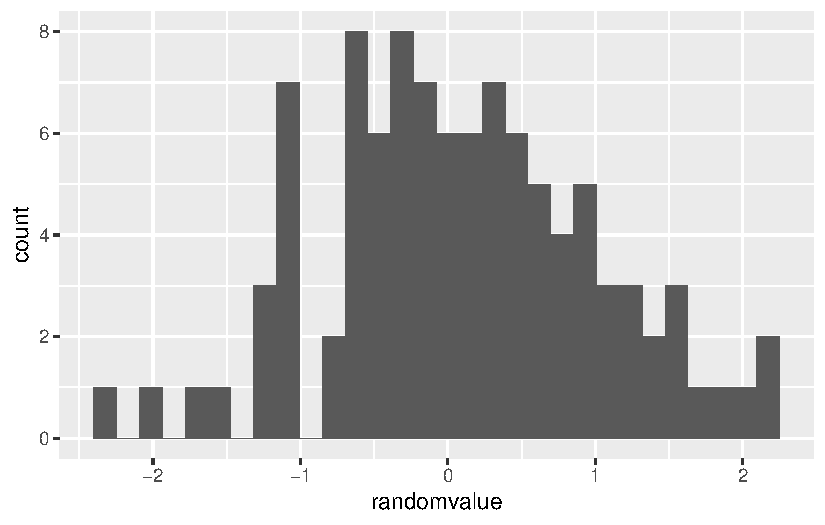
\includegraphics{01-working-with-quarto-qmd-scripts_files/figure-pdf/fig-histogram-1.pdf}

}

\caption{\label{fig-histogram}Histogram of 100 random values from a
normal distribution with 0 mean and 1 standard deviation}

\end{figure}%

So the text
```\texttt{\{r\}\ indicates\ that\ you\ start\ with\ a\ code\ chunk,\ and}```
completes it. use the quote that is typically the key below your
\textless esc\textgreater{} key on your keyboard. To keep your output
document clean, you can add options to messages and warnings (only add
when your codes works well)

\subsubsection{4. Redirect the output of a code
chunk}\label{redirect-the-output-of-a-code-chunk}

In the default settings of R Studio, the output of
Figure~\ref{fig-histogram} above is produced ``inline'', so in the the
same window where you read this now. This is fine for a final report or
supplement, but not desirable when developing the code. In that case, go
in R Studio to the menu Tools / Global Options / Markdown and uncheck
the option : ``Show output inline for all R Markdown documents''.\\
Then the output goes to the console and graph window, while this code
windows stays clean. You can also set it per script in the settings
option next to ``render'' in the small window menu bar above.

\subsubsection{5. Rendering a Quarto file to different types of
formatted
output}\label{rendering-a-quarto-file-to-different-types-of-formatted-output}

At the start of this .qmd file you find what is called the yaml header.
It contains information, using fixed field names, on the title, author
and data of the project.\\
A particularly important field for the next step is the output format
once the file is rendered.\\
For example, putting\\
format: docx\\
in the header renders to a Word docx file.\\
Some other options for output formats are:

\begin{longtable}[]{@{}ll@{}}
\toprule\noalign{}
Format: & Renders to: \\
\midrule\noalign{}
\endhead
\bottomrule\noalign{}
\endlastfoot
html & html for web pages (best default for viewing) \\
docx & Word file (best for copying to a document, report) \\
gfm & Github-friendly markdown (best for viewing on github) \\
PDF & Acrobat PDF (best for distributing) \\
mediawiki & native format for Wikipedia \\
\end{longtable}

Also see this \href{https://quarto.org/docs/reference/}{overview of
output formats}.

\subsubsection{6. Using different execution options in a code
chunk}\label{using-different-execution-options-in-a-code-chunk}

How a code chunk behaves is determined by the execution options. You can
set if you want different aspects as the code itself, the output from
that code, warnings, etc in the output document.

\begin{longtable}[]{@{}
  >{\raggedright\arraybackslash}p{(\columnwidth - 2\tabcolsep) * \real{0.2639}}
  >{\raggedright\arraybackslash}p{(\columnwidth - 2\tabcolsep) * \real{0.7361}}@{}}
\toprule\noalign{}
\begin{minipage}[b]{\linewidth}\raggedright
Execute option:
\end{minipage} & \begin{minipage}[b]{\linewidth}\raggedright
Descript
\end{minipage} \\
\midrule\noalign{}
\endhead
\bottomrule\noalign{}
\endlastfoot
eval & Evaluate the code chunk (if false, just echos the code into the
output). echo Include the source code in output \\
output & Include the results of executing the code in the output (true,
false, or asis to indicate that the output is raw markdown and should
not have any of Quarto's standard enclosing markdown). \\
warning & Include warnings in the output. \\
error & Include errors in the output (note that this implies that errors
executing code will not halt processing of the document). \\
include & Catch all for preventing any output (code or results) from
being included (e.g.~include: false suppresses all output from the code
block). \\
\end{longtable}

\subsubsection{7. Using formulas}\label{using-formulas}

Quarto syntax can also be used to generate equations as a Latex math
expression, for example

\[E = mc^{2}\]

Or, the cumulative distribution function of a normal distribution as
given by:

\[
\Phi(x) = \frac{1}{2} \left[ 1 + \operatorname{erf} \left( \frac{x - \mu}{\sigma \sqrt{2}} \right) \right]
\]

where: \(x\) is the variable \(\mu\) is the mean, \(\sigma\) is the
standard deviation, \(\operatorname{erf}(z)\) is the error function
defined by:

\[
\operatorname{erf}(z) = \frac{2}{\sqrt{\pi}} \int_0^z e^{-t^2} \, dt
\]



\end{document}
